\documentclass{beamer}
\graphicspath{ {../../instances/} }

%Information to be included in the title page:
\title{MAPF project}
\author{Andrés Córdova and Aleksandra Khatova}
\institute{Unversity of Potsdam}
\date{2022}

\AtBeginSection[]
{
  \begin{frame}
    \frametitle{Table of Contents}
    \tableofcontents[currentsection]
  \end{frame}
}

\begin{document}

\frame{\titlepage}

\begin{frame}
\frametitle{Traffic merger}
Common traffic rules: in case of conflict, turn to the right.
\end{frame}


\begin{frame}
\frametitle{Line merger}
\centering
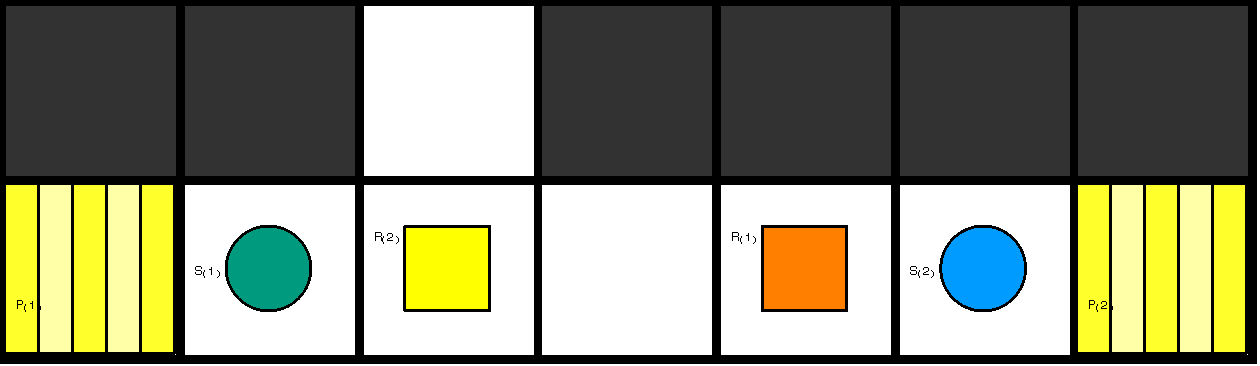
\includegraphics[scale=0.2]{x5y2r2s2p2.png}
\end{frame}

\begin{frame}
\frametitle{Automation}
Script run\_clingo.py allows to launch the pipeline using a single command
\end{frame}

\begin{frame}
\frametitle{Modules}
\begin{itemize}
\item<1->asprilo\_output\_to\_input.lp: Translates "occurs" into position and move
\item<2->conflicts\_detector.lp: Finds and classifies conflicts
\item<3->action.lp: Basic movement rules (e.g., robot must stay on the grid)
\item<4->merger\_output.lp: Formats the output
\item<4->Different merger modules
\end{itemize}
\end{frame}


\begin{frame}
\frametitle{Further work}
\begin{itemize} 
\item<1-> Automate creation of separate plans for each robot using asprilo
\item<2-> Define our long-term goals: what will be special about our project?
\item<3-> Try other merging strategies, especially the more difficult ones
\end{itemize} 
\end{frame}



\end{document}